\documentclass
[
    a4paper,
    11pt,
    bibliography = totoc,
    listof = totoc,
    headinclude = true,
]
{scrreport}

\parindent=0pt
% Hier befinden sich Pakete, die wir beinahe immer benutzen ...

\usepackage[utf8]{inputenc}

% Sprach-Paket:
\usepackage[english]{babel}

% damit's nicht so, wie beim Grill aussieht:
\usepackage{fullpage}
\usepackage{changepage}

% Mathematik:
\usepackage{amsmath, amssymb, amsfonts, amsthm}
\usepackage{bbm, mathrsfs, stmaryrd}
\usepackage{mathtools, mathdots}

% Doppel-Klammern:
\usepackage{stmaryrd}

% Makros mit mehereren Default-Argumenten:
\usepackage{twoopt}

% Anführungszeichen (Makro \Quote{}):
\usepackage{babel}

% if's für Makros:
\usepackage{xifthen}
\usepackage{etoolbox}

% *'s für Makros:
\usepackage{suffix}

% tikz ist kein Zeichenprogramm (doch!):
\usepackage{tikz}
\usetikzlibrary{arrows}
\usetikzlibrary{decorations.markings}

% bessere Aufzählungen:
\usepackage{enumitem}

% (bessere) Umgebung für Bilder:
\usepackage{graphicx, subfig, float}
\usepackage{tcolorbox}

% Umgebung für Code:
\usepackage{listings}

% Farben:
\usepackage{xcolor}

% Umgebung für "plain text":
\usepackage{verbatim}

% Umgebung für mehrerer Spalten:
\usepackage{multicol}
\setlength{\columnsep}{1cm}

% diagonale Brüche
\usepackage{nicefrac}

% faktorisieren
\usepackage{faktor}

% Spaltentypen verschiedener Dicke
\usepackage{tabularx}
\usepackage{makecell}

% Für Vektoren
\usepackage{esvect}

% (Web-)Links
\usepackage{hyperref}

% Zitieren & Literatur-Verzeichnis
\usepackage[
backend=biber,
style=numeric
]{biblatex}
\usepackage{csquotes}

% so ähnlich wie mathbb
%\usepackage{mathds}

% Keine Ahnung, was das macht ...
\usepackage{booktabs}
\usepackage{ngerman}
\usepackage{placeins}

% Bäume
\usepackage[noeepic]{qtree}

% Algorithmen
\usepackage{algorithm}
\usepackage{algpseudocode}

% special letters:

\newcommand{\N}{\mathbb{N}}
\newcommand{\Z}{\mathbb{Z}}
\newcommand{\Q}{\mathbb{Q}}
\newcommand{\R}{\mathbb{R}}
\newcommand{\C}{\mathbb{C}}
\newcommand{\K}{\mathbb{K}}
\newcommand{\T}{\mathbb{T}}
\newcommand{\E}{\mathbb{E}}
\newcommand{\V}{\mathbb{V}}
\renewcommand{\S}{\mathbb{S}}
\renewcommand{\P}{\mathbb{P}}
\newcommand{\1}{\mathbbm{1}}

% quantors:

\newcommand{\Forall}{\forall \,}
\newcommand{\Exists}{\exists \,}
\newcommand{\ExistsOnlyOne}{\exists! \,}
\newcommand{\nExists}{\nexists \,}
\newcommand{\ForAlmostAll}{\forall^\infty \,}

% MISC symbols:

\newcommand{\landau}{{\scriptstyle \mathcal{O}}}
\newcommand{\Landau}{\mathcal{O}}


\newcommand{\eps}{\mathrm{eps}}

% graphics in a box:

\newcommandtwoopt
{\includegraphicsboxed}[3][][]
{
  \begin{figure}[!h]
    \begin{boxedin}
      \ifthenelse{\isempty{#1}}
      {
        \begin{center}
          \includegraphics[width = 0.75 \textwidth]{#3}
          \label{fig:#2}
        \end{center}
      }{
        \begin{center}
          \includegraphics[width = 0.75 \textwidth]{#3}
          \caption{#1}
          \label{fig:#2}
        \end{center}
      }
    \end{boxedin}
  \end{figure}
}

% braces:

\newcommand{\pbraces}[1]{{\left  ( #1 \right  )}}
\newcommand{\bbraces}[1]{{\left  [ #1 \right  ]}}
\newcommand{\Bbraces}[1]{{\left \{ #1 \right \}}}
\newcommand{\vbraces}[1]{{\left  | #1 \right  |}}
\newcommand{\Vbraces}[1]{{\left \| #1 \right \|}}
\newcommand{\abraces}[1]{{\left \langle #1 \right \rangle}}
\newcommand{\round}[1]{\bbraces{#1}}

\newcommand
{\floorbraces}[1]
{{\left \lfloor #1 \right \rfloor}}

\newcommand
{\ceilbraces} [1]
{{\left \lceil  #1 \right \rceil }}

% special functions:

\newcommand{\norm}  [2][]{\Vbraces{#2}_{#1}}
\newcommand{\diam}  [2][]{\mathrm{diam}_{#1} \: #2}
\newcommand{\diag}  [1]{\mathrm{diag} \: #1}
\newcommand{\dist}  [1]{\mathrm{dist} \: #1}
\newcommand{\mean}  [1]{\mathrm{mean} \: #1}
\newcommand{\erf}   [1]{\mathrm{erf} \: #1}
\newcommand{\id}    [1]{\mathrm{id} \: #1}
\newcommand{\sgn}   [1]{\mathrm{sgn} \: #1}
\newcommand{\supp}  [1]{\mathrm{supp} \: #1}
\newcommand{\arsinh}[1]{\mathrm{arsinh} \: #1}
\newcommand{\arcosh}[1]{\mathrm{arcosh} \: #1}
\newcommand{\artanh}[1]{\mathrm{artanh} \: #1}
\newcommand{\card}  [1]{\mathrm{card} \: #1}
\newcommand{\Span}  [1]{\mathrm{span} \: #1}
\newcommand{\Aut}   [1]{\mathrm{Aut} \: #1}
\newcommand{\End}   [1]{\mathrm{End} \: #1}
\newcommand{\ggT}   [1]{\mathrm{ggT} \: #1}
\newcommand{\kgV}   [1]{\mathrm{kgV} \: #1}
\newcommand{\ord}   [1]{\mathrm{ord} \: #1}
\newcommand{\grad}  [1]{\mathrm{grad} \: #1}
\newcommand{\ran}   [1]{\mathrm{ran} \: #1}
\newcommand{\graph} [1]{\mathrm{graph} \: #1}
\newcommand{\Inv}   [1]{\mathrm{Inv} \: #1}
\newcommand{\pv}    [1]{\mathrm{pv} \: #1}
\newcommand{\GL}    [1]{\mathrm{GL} \: #1}
\newcommand{\Mod}{\mathrm{Mod} \:}
\newcommand{\Th}{\mathrm{Th} \:}
\newcommand{\Char}{\mathrm{char}}
\newcommand{\At}{\mathrm{At}}
\newcommand{\Ob}{\mathrm{Ob}}
\newcommand{\Hom}{\mathrm{Hom}}
\newcommand{\orthogonal}[3][]{#2 ~\bot_{#1}~ #3}
\newcommand{\Rang}{\mathrm{Rang}}
\newcommand{\NIL}{\mathrm{NIL}}
\newcommand{\Res}{\mathrm{Res}}
\newcommand{\lxor}{\dot \lor}
\newcommand{\Div}{\mathrm{div} \:}
\newcommand{\meas}{\mathrm{meas} \:}

% fractions:

\newcommand{\Frac}[2]{\frac{1}{#1} \pbraces{#2}}
\newcommand{\nfrac}[2]{\nicefrac{#1}{#2}}

% derivatives & integrals:

\newcommandtwoopt
{\Int}[4][][]
{\int_{#1}^{#2} #3 ~\mathrm{d} #4}

\newcommandtwoopt
{\derivative}[3][][]
{
  \frac
  {\mathrm{d}^{#1} #2}
  {\mathrm{d} #3^{#1}}
}

\newcommandtwoopt
{\pderivative}[3][][]
{
  \frac
  {\partial^{#1} #2}
  {\partial #3^{#1}}
}

\newcommand
{\primeprime}
{{\prime \prime}}

\newcommand
{\primeprimeprime}
{{\prime \prime \prime}}

% Text:

\newcommand{\Quote}[1]{\glqq #1\grqq{}}
\newcommand{\Text}[1]{{\text{#1}}}
\newcommand{\fastueberall}{\text{f.ü.}}
\newcommand{\fastsicher}{\text{f.s.}}

% ---------------------------------------------------------------- %
% amsthm-environments:

\theoremstyle{definition}

% numbered theorems
\newtheorem{theorem}             {Theorem}[section]
\newtheorem{lemma}      [theorem]{Lemma}
\newtheorem{corollary}  [theorem]{Corollary}
\newtheorem{proposition}[theorem]{Proposition}
\newtheorem{remark}     [theorem]{Remark}
\newtheorem{definition} [theorem]{Definition}
\newtheorem{example}    [theorem]{Example}
\newtheorem{heuristics} [theorem]{Heuristics}

% unnumbered theorems
\newtheorem*{theorem*}    {Theorem}
\newtheorem*{lemma*}      {Lemma}
\newtheorem*{corollary*}  {Corollary}
\newtheorem*{proposition*}{Proposition}
\newtheorem*{remark*}     {Remark}
\newtheorem*{definition*} {Definition}
\newtheorem*{example*}    {Example}
\newtheorem*{heuristics*} {Heuristics}

% ---------------------------------------------------------------- %
% exercise- and solution-environments:

% Please define this stuff in project ("main.tex"):
% \def \lastexercisenumber {...}

\newtheorem{exercise}{Exercise}
\setcounter{exercise}{\lastexercisenumber}

\newenvironment{solution}
{
  \begin{proof}[Solution]
}{
  \end{proof}
}

% ---------------------------------------------------------------- %
% MISC translations for environment-names

\renewcommand{\proofname} {Proof}
\renewcommand{\figurename}{Figure}
\renewcommand{\tablename} {Table}

% ---------------------------------------------------------------- %

% ---------------------------------------------------------------- %
% https://www.overleaf.com/learn/latex/Code_listing

\definecolor{codegreen} {rgb}{0, 0.6, 0}
\definecolor{codegray}    {rgb}{0.5, 0.5, 0.5}
\definecolor{codepurple}{rgb}{0.58, 0, 0.82}
\definecolor{backcolour}{rgb}{0.95, 0.95, 0.92}

\lstdefinestyle{overleaf}
{
    backgroundcolor = \color{backcolour},
    commentstyle = \color{codegreen},
    keywordstyle = \color{magenta},
    numberstyle = \tiny\color{codegray},
    stringstyle = \color{codepurple},
    basicstyle = \ttfamily \footnotesize,
    breakatwhitespace = false,
    breaklines = true,
    captionpos = b,
    keepspaces = true,
    numbers = left,
    numbersep = 5pt,
    showspaces = false,
    showstringspaces = false,
    showtabs = false,
    tabsize = 2
}

% ---------------------------------------------------------------- %
% https://en.wikibooks.org/wiki/LaTeX/Source_Code_Listings

\lstdefinestyle{customc}
{
    belowcaptionskip = 1 \baselineskip,
    breaklines = true,
    frame = L,
    xleftmargin = \parindent,
    language = C,
    showstringspaces = false,
    basicstyle = \footnotesize \ttfamily,
    keywordstyle = \bfseries \color{green!40!black},
    commentstyle = \itshape \color{purple!40!black},
    identifierstyle = \color{blue},
    stringstyle = \color{orange},
}

\lstdefinestyle{customasm}
{
    belowcaptionskip = 1 \baselineskip,
    frame = L,
    xleftmargin = \parindent,
    language = [x86masm] Assembler,
    basicstyle = \footnotesize\ttfamily,
    commentstyle = \itshape\color{purple!40!black},
}

% ---------------------------------------------------------------- %
% https://tex.stackexchange.com/questions/235731/listings-syntax-for-literate

\definecolor{maroon}        {cmyk}{0, 0.87, 0.68, 0.32}
\definecolor{halfgray}      {gray}{0.55}
\definecolor{ipython_frame} {RGB}{207, 207, 207}
\definecolor{ipython_bg}    {RGB}{247, 247, 247}
\definecolor{ipython_red}   {RGB}{186, 33, 33}
\definecolor{ipython_green} {RGB}{0, 128, 0}
\definecolor{ipython_cyan}  {RGB}{64, 128, 128}
\definecolor{ipython_purple}{RGB}{170, 34, 255}

\lstdefinestyle{stackexchangePython}
{
    breaklines = true,
    %
    extendedchars = true,
    literate =
    {á}{{\' a}} 1 {é}{{\' e}} 1 {í}{{\' i}} 1 {ó}{{\' o}} 1 {ú}{{\' u}} 1
    {Á}{{\' A}} 1 {É}{{\' E}} 1 {Í}{{\' I}} 1 {Ó}{{\' O}} 1 {Ú}{{\' U}} 1
    {à}{{\` a}} 1 {è}{{\` e}} 1 {ì}{{\` i}} 1 {ò}{{\` o}} 1 {ù}{{\` u}} 1
    {À}{{\` A}} 1 {È}{{\' E}} 1 {Ì}{{\` I}} 1 {Ò}{{\` O}} 1 {Ù}{{\` U}} 1
    {ä}{{\" a}} 1 {ë}{{\" e}} 1 {ï}{{\" i}} 1 {ö}{{\" o}} 1 {ü}{{\" u}} 1
    {Ä}{{\" A}} 1 {Ë}{{\" E}} 1 {Ï}{{\" I}} 1 {Ö}{{\" O}} 1 {Ü}{{\" U}} 1
    {â}{{\^ a}} 1 {ê}{{\^ e}} 1 {î}{{\^ i}} 1 {ô}{{\^ o}} 1 {û}{{\^ u}} 1
    {Â}{{\^ A}} 1 {Ê}{{\^ E}} 1 {Î}{{\^ I}} 1 {Ô}{{\^ O}} 1 {Û}{{\^ U}} 1
    {œ}{{\oe}}  1 {Œ}{{\OE}}  1 {æ}{{\ae}}  1 {Æ}{{\AE}}  1 {ß}{{\ss}}  1
    {ç}{{\c c}} 1 {Ç}{{\c C}} 1 {ø}{{\o}} 1 {å}{{\r a}} 1 {Å}{{\r A}} 1
    {€}{{\EUR}} 1 {£}{{\pounds}} 1
}


% Python definition (c) 1998 Michael Weber
% Additional definitions (2013) Alexis Dimitriadis
% modified by me (should not have empty lines)

\lstdefinelanguage{iPython}{
    morekeywords = {access, and, break, class, continue, def, del, elif, else, except, exec, finally, for, from, global, if, import, in, is, lambda, not, or, pass, print, raise, return, try, while}, %
    %
    % Built-ins
    morekeywords = [2]{abs, all, any, basestring, bin, bool, bytearray, callable, chr, classmethod, cmp, compile, complex, delattr, dict, dir, divmod, enumerate, eval, execfile, file, filter, float, format, frozenset, getattr, globals, hasattr, hash, help, hex, id, input, int, isinstance, issubclass, iter, len, list, locals, long, map, max, memoryview, min, next, object, oct, open, ord, pow, property, range, raw_input, reduce, reload, repr, reversed, round, set, setattr, slice, sorted, staticmethod, str, sum, super, tuple, type, unichr, unicode, vars, xrange, zip, apply, buffer, coerce, intern}, %
    %
    sensitive = true, %
    morecomment = [l] \#, %
    morestring = [b]', %
    morestring = [b]", %
    %
    morestring = [s]{'''}{'''}, % used for documentation text (mulitiline strings)
    morestring = [s]{"""}{"""}, % added by Philipp Matthias Hahn
    %
    morestring = [s]{r'}{'},     % `raw' strings
    morestring = [s]{r"}{"},     %
    morestring = [s]{r'''}{'''}, %
    morestring = [s]{r"""}{"""}, %
    morestring = [s]{u'}{'},     % unicode strings
    morestring = [s]{u"}{"},     %
    morestring = [s]{u'''}{'''}, %
    morestring = [s]{u"""}{"""}, %
    %
    % {replace}{replacement}{lenght of replace}
    % *{-}{-}{1} will not replace in comments and so on
    literate = 
    {á}{{\' a}} 1 {é}{{\' e}} 1 {í}{{\' i}} 1 {ó}{{\' o}} 1 {ú}{{\' u}} 1
    {Á}{{\' A}} 1 {É}{{\' E}} 1 {Í}{{\' I}} 1 {Ó}{{\' O}} 1 {Ú}{{\' U}} 1
    {à}{{\` a}} 1 {è}{{\` e}} 1 {ì}{{\` i}} 1 {ò}{{\` o}} 1 {ù}{{\` u}} 1
    {À}{{\` A}} 1 {È}{{\' E}} 1 {Ì}{{\` I}} 1 {Ò}{{\` O}} 1 {Ù}{{\` U}} 1
    {ä}{{\" a}} 1 {ë}{{\" e}} 1 {ï}{{\" i}} 1 {ö}{{\" o}} 1 {ü}{{\" u}} 1
    {Ä}{{\" A}} 1 {Ë}{{\" E}} 1 {Ï}{{\" I}} 1 {Ö}{{\" O}} 1 {Ü}{{\" U}} 1
    {â}{{\^ a}} 1 {ê}{{\^ e}} 1 {î}{{\^ i}} 1 {ô}{{\^ o}} 1 {û}{{\^ u}} 1
    {Â}{{\^ A}} 1 {Ê}{{\^ E}} 1 {Î}{{\^ I}} 1 {Ô}{{\^ O}} 1 {Û}{{\^ U}} 1
    {œ}{{\oe}}  1 {Œ}{{\OE}}  1 {æ}{{\ae}}  1 {Æ}{{\AE}}  1 {ß}{{\ss}}  1
    {ç}{{\c c}} 1 {Ç}{{\c C}} 1 {ø}{{\o}} 1 {å}{{\r a}} 1 {Å}{{\r A}} 1
    {€}{{\EUR}} 1 {£}{{\pounds}} 1
    %
    {^}{{{\color{ipython_purple}\^ {}}}} 1
    { = }{{{\color{ipython_purple} = }}} 1
    %
    {+}{{{\color{ipython_purple}+}}} 1
    {*}{{{\color{ipython_purple}$^\ast$}}} 1
    {/}{{{\color{ipython_purple}/}}} 1
    %
    {+=}{{{+=}}} 1
    {-=}{{{-=}}} 1
    {*=}{{{$^\ast$ = }}} 1
    {/=}{{{/=}}} 1,
    literate = 
    *{-}{{{\color{ipython_purple} -}}} 1
     {?}{{{\color{ipython_purple} ?}}} 1,
    %
    identifierstyle = \color{black}\ttfamily,
    commentstyle = \color{ipython_cyan}\ttfamily,
    stringstyle = \color{ipython_red}\ttfamily,
    keepspaces = true,
    showspaces = false,
    showstringspaces = false,
    %
    rulecolor = \color{ipython_frame},
    frame = single,
    frameround = {t}{t}{t}{t},
    framexleftmargin = 6mm,
    numbers = left,
    numberstyle = \tiny\color{halfgray},
    %
    %
    backgroundcolor = \color{ipython_bg},
    % extendedchars = true,
    basicstyle = \scriptsize,
    keywordstyle = \color{ipython_green}\ttfamily,
}

% ---------------------------------------------------------------- %
% https://tex.stackexchange.com/questions/417884/colour-r-code-to-match-knitr-theme-using-listings-minted-or-other

\geometry{verbose, tmargin = 2.5cm, bmargin = 2.5cm, lmargin = 2.5cm, rmargin = 2.5cm}

\definecolor{backgroundCol}  {rgb}{.97, .97, .97}
\definecolor{commentstyleCol}{rgb}{0.678, 0.584, 0.686}
\definecolor{keywordstyleCol}{rgb}{0.737, 0.353, 0.396}
\definecolor{stringstyleCol} {rgb}{0.192, 0.494, 0.8}
\definecolor{NumCol}         {rgb}{0.686, 0.059, 0.569}
\definecolor{basicstyleCol}  {rgb}{0.345, 0.345, 0.345}

\lstdefinestyle{stackexchangeR}
{
    language = R,                                        % the language of the code
    basicstyle = \small \ttfamily \color{basicstyleCol}, % the size of the fonts that are used for the code
    % numbers = left,                                      % where to put the line-numbers
    numberstyle = \color{green},                         % the style that is used for the line-numbers
    stepnumber = 1,                                      % the step between two line-numbers. If it is 1, each line will be numbered
    numbersep = 5pt,                                     % how far the line-numbers are from the code
    backgroundcolor = \color{backgroundCol},             % choose the background color. You must add \usepackage{color}
    showspaces = false,                                  % show spaces adding particular underscores
    showstringspaces = false,                            % underline spaces within strings
    showtabs = false,                                    % show tabs within strings adding particular underscores
    % frame = single,                                      % adds a frame around the code
    % rulecolor = \color{white},                           % if not set, the frame-color may be changed on line-breaks within not-black text (e.g. commens (green here))
    tabsize = 2,                                         % sets default tabsize to 2 spaces
    captionpos = b,                                      % sets the caption-position to bottom
    breaklines = true,                                   % sets automatic line breaking
    breakatwhitespace = false,                           % sets if automatic breaks should only happen at whitespace
    keywordstyle = \color{keywordstyleCol},              % keyword style
    commentstyle = \color{commentstyleCol},              % comment style
    stringstyle = \color{stringstyleCol},                % string literal style
    literate = %
    *{0}{{{\color{NumCol} 0}}} 1
     {1}{{{\color{NumCol} 1}}} 1
     {2}{{{\color{NumCol} 2}}} 1
     {3}{{{\color{NumCol} 3}}} 1
     {4}{{{\color{NumCol} 4}}} 1
     {5}{{{\color{NumCol} 5}}} 1
     {6}{{{\color{NumCol} 6}}} 1
     {7}{{{\color{NumCol} 7}}} 1
     {8}{{{\color{NumCol} 8}}} 1
     {9}{{{\color{NumCol} 9}}} 1
}

% ---------------------------------------------------------------- %
% Fundament Mathematik

\lstdefinestyle{fundament}{basicstyle = \ttfamily}

% ---------------------------------------------------------------- %


\addbibresource{Quellen/references.bib}

\begin{document}

\subject{Modeling \& Simulation}
\title{SIR Model - Mass Tests}

\publishers{Betreuer: Martin Bicher }


\author{
Christian Göth \and
Christian Sallinger \and
Florian Schager \and
Paul Winkler
}


\maketitle

\chapter*{Abstract}

In 2020 the COVID-19 pandemic caused worldwide suffering and deaths and the
whole world is waiting for a vaccine. In winter 2020/2021 countries in Europe
came up with the idea of executing nationwide mass tests to reduce the number
of unconfirmed cases. This strategy should serve as an alternative to
lockdown measures that force people to reduce their contacts.
In this project we want to contrast these alternatives qualitatively and quantitatively
by constructing a modified SIR Model to simulate the spread of the disease.
With our model we want to answer the question:
How many days of lockdown are necessary with different strategies of mass-testing?


\tableofcontents


\chapter{Model Description}

Our model is based on the classical SIR Model by Kermack and McKendrick,
but in addition to the standard compartments Susceptible, Infectious, Recovered
we introduce an extra Exposed compartment between the Susceptible and the Infectious.
Furthermore we split the Infectious compartment into two seperate compartments:
Confirmed and Unconfirmed. \\
In our model we assume, that the persons in the Confirmed compartment are in
quarantine and do not contribute to the infection rate anymore.
To capture the causal relations within our model we first sketch a basic
causal loop diagram.

\section{Causal Loop Diagram}

As one can see in the figure below, there are two main balancing loops
in our model and one reinforcing loop. The upper balancing loop only
becomes relevant after a big portion of the population has already recovered
from the virus and therefore our model will focus on how the disease can
be controlled with different strategies of countermeasures.

\begin{figure}[hbt!]
  \caption{Causal Loop Diagram}
  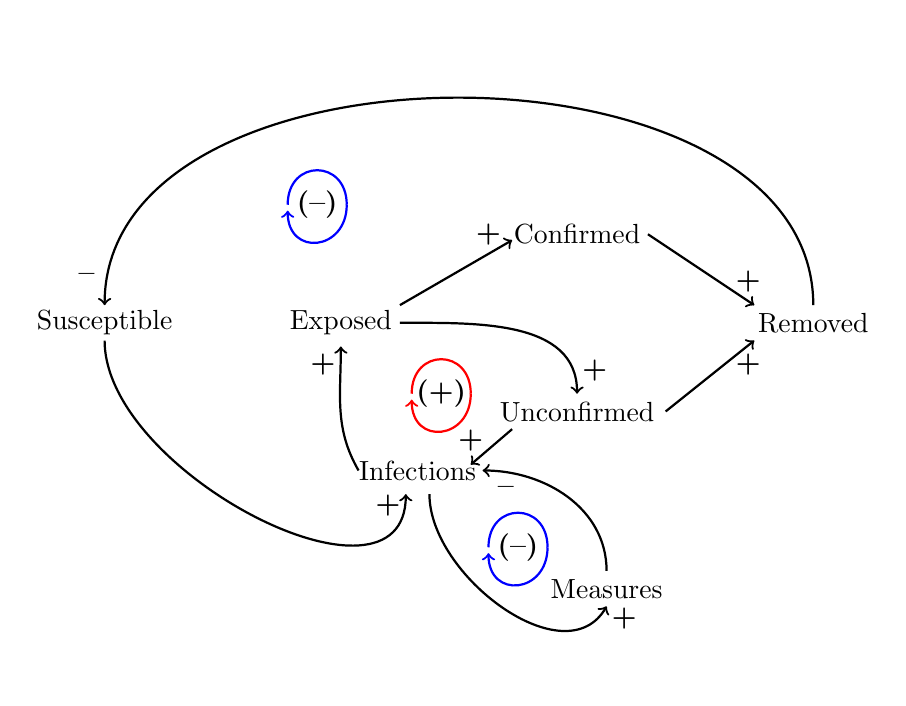
\begin{tikzpicture}[scale=0.75]
\draw[->, thick] (0.5,-2.9) to [out=-90, in=-120] (3.5,-4.8);
\draw[->, thick] (3.5,-4.2) to [out=90, in=0] (1.4,-2.5);
  \draw[->, thick] (-5,-0.3) to [out=-90, in=-90] (0.1,-2.9);
  \draw[->, thick] (0,0.3) -- (1.9,1.4);
  \draw[->, thick] (0,0) to [out=0,in=90] (3,-1.2);

  \draw[->, thick] (4.2,1.5) -- (6,0.3);
  \draw[->, thick] (4.5,-1.5) -- (6,-0.3);
\draw [->, thick] (1.9, -1.8) -- (1.2,-2.4);
 \draw [->, thick] (-0.7, -2.5) to [out=120,in=-90] (-1,-0.4);
\draw [->, thick] (7, 0.3) to [out=90,in=90] (-5,0.3);


\draw [thick, blue] (-1.9,2) to [out=90,in=90, looseness=2] (-0.9,2);
\draw [->, thick, blue] (-0.9,2) to [out=-90,in=-90, looseness=2] (-1.9,1.9);
  \node[very thick] at (-1.4,2) {\textbf{(--)}};

 \draw [thick, red] (0.2,-1.2) to [out=90,in=90, looseness=2] (1.2,-1.2);
\draw [->, thick, red] (1.2,-1.2) to [out=-90,in=-90, looseness=2] (0.2, -1.3);
  \node[very thick] at (0.7,-1.2) {\textbf{(+)}};

 \draw [thick, blue] (1.5,-3.8) to [out=90,in=90, looseness=2] (2.5,-3.8);
\draw [->, thick, blue] (2.5,-3.8) to [out=-90,in=-90, looseness=2] (1.5, -3.9);
  \node[very thick] at (2,-3.8) {\textbf{(--)}};

  \node[very thick] at (1.2,-2) {\textbf{+}};
  \node[very thick] at (1.8,-2.8) {\textbf{--}};
  \node[very thick] at (-0.2,-3.1) {\textbf{+}};
  \node[very thick] at (1.5,1.5) {\textbf{+}};
  \node[very thick] at (3.3,-0.8) {\textbf{+}};
  \node[very thick] at (5.9,0.7) {\textbf{+}};
  \node[very thick] at (5.9,-0.7) {\textbf{+}};
  \node[very thick] at (-5.3,0.8) {\textbf{--}};
  \node[very thick] at (-1.3,-0.7) {\textbf{+}};
  \node[very thick] at (3.8,-5) {\textbf{+}};
  \node[draw = none] at (-5,0) {Susceptible};
  \node[draw = none] at (-1,0) {Exposed};
  \node[draw = none] at (3,1.5) {Confirmed};
  \node[draw = none] at (3,-1.5) {Unconfirmed};
  \node[draw = none] at (7,0) {Removed};
  \node[draw = none] at (0.3,-2.5) {Infections};
  \node[draw = none] at (3.5,-4.5) {Measures};

\end{tikzpicture}

\end{figure}

\section{Stock and Flow Diagram}

For the Stock and Flow Diagram of our model we jump directly into
our AnyLogic-Implementation. As already mentioned, the stocks in our model
are the Susceptible, Exposed, Confirmed, Unconfirmed and Recovered compartments.

\begin{figure}[hbt!]
  \caption{Stock and Flow Diagram}
  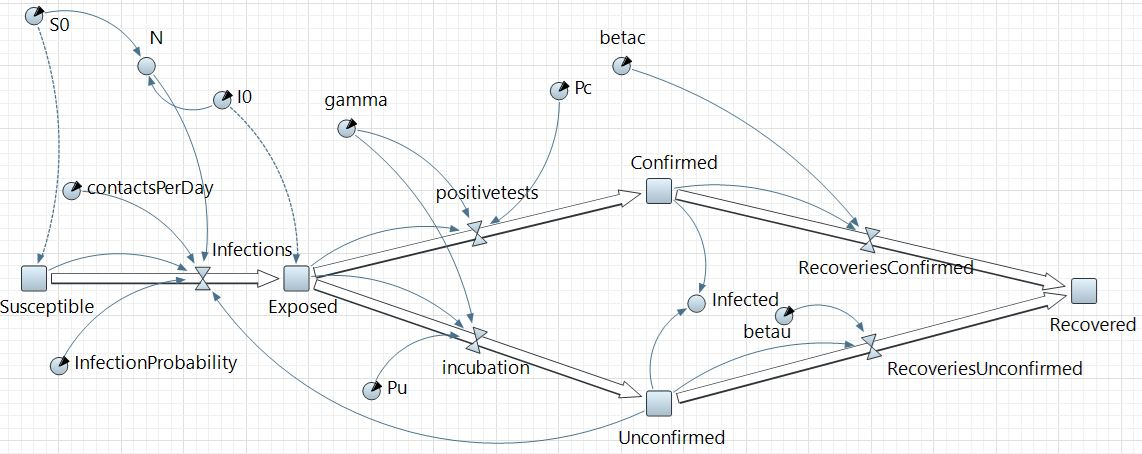
\includegraphics[width=\linewidth]{../AnyLogicSIR.JPG}
\end{figure}

\FloatBarrier

\section{Parameters}

We choose our contactsPerDay to be 12 before the start of the pandemic,
based on \cite{Spiegel}. With our lockdown events, which we will discuss
later, this value will vary through the course of the pandemic.
Inseperably intertwined with the contactsPerDay parameter is our parameter
for the InfectionProbability. Since our formula for the Infections states

\begin{align*}
  \text{Infections} = \text{Susceptible} \cdot \text{contactsPerDay} \cdot
  \text{InfectionProbability} \cdot
  \text{Unconfirmed} \cdot \frac{1}{N},
\end{align*}

a change in the first parameter would have the same effect on our model
as the analogous change in the second parameter.
This posed the challenging task of finding realistic values for those parameters.
Therefore we determined our parameter for the InfectionProbability by comparing
our model results with the data provided by \cite{OrfCorona} and finally
settled for the baseline

\begin{align*}
  \text{InfectionProbability} = 0.06.
\end{align*}

Furthermore to reflect the seasonal differences in the course of the pandemic,
we lowered the InfectionProbability in the summer to $0.02$. \\
Next we needed to determine the value of gamma, which is determined by the time
it takes from contracting the virus to becoming infectious oneself.
We refer to \cite{RobertKochInstitut}, where a feasible parameter value of $5$ is given. \\
For the rate of positive tests, we took a look at the current state in Austria,
where approximately $65\%$ of infection go by unnoticed \cite{MassTests}.
Of course one constant value for the rate of positive tests cannot perfectly
modeled an ever changing pandemic, however, continuously changing the value
throughout the pandemic seemed to be a too daunting task to handle. \\
For the recovery parameter the only value that truly matters in our model
is the recovery rate for the Unconfirmed compartment, since the people in the
Confirmed compartment already do not contribute to the spread of the pandemic anymore.
For the value of RecoveriesUnconfirmed we oriented us on the average number of days
it takes to recover from the virus, which we assumed to be around $7$ days.
The inverse of this value roughly yield our parameter value of

\begin{align*}
  \beta_u = 0.15.
\end{align*}

Finally we address the starting values for our model. We choose our start date
to be the 25th of February 2020 and assume an initial 300 infections.
Our parameter for $N$ is simply chosen as the current population of Austria,
which yields the approximate value of $N = 8,900,000$.
We end our simulation on 28.01.2022, exactly one year after the presentation date.

\section{Events}

First of all, we of course implemented a mass test event. In our implementation
this immediately transfers a predefined fraction of our Unconfirmed compartment
to the Confirmed compartment. In addition to this instanteous shift we also
adjusted the rate of confirmed cases for the next three days after the start of
the mass test accordingly. We experimented with different participation rates
for our masstests, starting from $25\%$, roughly the average participation rate
for the previous masstests in Austria, all the way up to the illusive rate of $90\%$.
For the recurrence of the masstests, we implemented them to occur cyclically,
experimenting again with different time intervals for the cycle. The first masstest
starts on the 12th of December, just like in reality.\\

The second big event we implemented was of course the Lockdown. To be precise,
we modeled multiple different version of Lockdowns, but all with the same basic idea:
The Lockdowns triggers, once the number of Infected people (Confirmed and Unconfirmed combined)
reaches a certain level. Precise numbers for this are found in the table below.
We chose the value of Infected people over the value of
the Confirmed people as the main indicator for our model Lockdown, even though
in reality only the number of Confirmed people is accurately known.
Our reasoning for this was, that the total number of Infected people in our
model should be the best indicator for the strain of the virus on our health system,
which would be a major deciding factor in the decision to implement a Lockdown in reality.
The effect of a Lockdown in our model is simply a reduction of the contactsPerDay parameter.
To account for the multiple levels of reopening like we have seen in previous
lockdown, we implemented different levels of lockdown, which gradually increase
the number of contactsPerDay to pre-pandemic levels.
\begin{table}[!h]
  \begin{center}
  \begin{tabular}{|c||c|c|c|c|}
  \hline
    Nr. Infected &- & $\geq 45,000$ & $\leq 10,000$ & $\leq 5,000$ \\
    \hline
    contacts per Day & 14 & 2 & 6 & 9 \\
    \hline
  \end{tabular}
  \end{center}
  \caption{Numbers for first lockdown}
\end{table}

\begin{table}[!h]
  \begin{center}
  \begin{tabular}{|c||c|c|c|c|}
  \hline
    Nr. Infected &- & $\geq 115,000$ & $\leq 30,000$ & $\leq 20,000$ \\
    \hline
    contacts per Day & 9 & 3 & 6 & 9 \\
    \hline
  \end{tabular}
  \end{center}
  \caption{Numbers for other lockdowns}
\end{table}

\chapter{Simulation Results}

To compare the different masstest parameters we measured the amount of days in
Lockdown after December 12th. To do this we created a different stock and assumed
a flow of $1$ during a lockdown and $0.5$ during the first level of reopening.
\begin{table}[!h]
{\small%
\begin{center}
\begin{tabular}{|c||c|c|c|c|}
\hline
& 30 days    & 21 days   & 14 days  & 7 days  \\
 \hline
 \hline
     $25\%$ participation & 119 &96 & 86 & 60\\
 \hline
     $35\%$ participation & 96 &  86&  78  & 36   \\
 \hline
     $50\%$ participation & 86 & 77 & 49 & 5\\
 \hline
     $70\%$ participation & 75 &  45 & 6 & 4 \\
 \hline
     $90\%$ participation & 39 &4 &4  & 3\\
     \hline
\end{tabular}
\end{center}
}%

\caption{Days of lockdown with different participation rate and interval between masstests}
\end{table} \\
To compare: without any masstests at all the number of days in lockdown would be
$156$. The actual participation rate ranged from $14-36\%$ (averageing about $25\%$), depending on state, with the lowest rate in Vienna and the highest in Lower Austria. The first two masstests happened in the middle of December and January, respectively, so the parameters that best fit reality would be the $25\%$ participation with a $30$ day interval between the masstests.

Our simulation now suggests that to really get the most out of masstesting we would need to either heavily increase the participation rate or decrease the interval between masstests, ideally both. \\

One thing we want to stress is, that in our model no vaccinations are done at all. Since the first vaccinations are already happening right now our model might make the situation look more grim than it really is.
\end{document}
